% This is LLNCS.DEM the demonstration file of
% the LaTeX macro package from Springer-Verlag
% for Lecture Notes in Computer Science,
% version 2.4 for LaTeX2e as of 16. April 2010
%
\documentclass{llncs}

\usepackage{graphicx}
\usepackage[utf8]{inputenc}
%\usepackage[T1]{fontenc}

\usepackage{booktabs}
\usepackage{multirow}

%
\begin{document}


\newcommand{\tk}[1]{{
   \bf
   [TK\footnote{Anmerkung TK: #1}]
}}

\newcommand{\regie}[1]{
   \rule{0mm}{0mm} \hfill
   \framebox{
      \begin{minipage}[b]{0.8\linewidth}
         {\tt #1}
      \end{minipage}
   }
} 


\title{Applying Higher-Order Model Transformations to the Semantic Lifting of Model Differences}

\author{Timo Kehrer, Manuel Ohrndorf, Udo Kelter and Maik Schmidt}

\institute{Software Engineering Group\\University of Siegen, Germany\\
\email{\{kehrer,mohrndorf,kelter,mschmidt\}@informatik.uni-siegen.de}
}

% \institute{Princeton University, Princeton NJ 08544, USA,\\
% \email{I.Ekeland@princeton.edu},\\ WWW home page:
% \texttt{http://users/\homedir iekeland/web/welcome.html}
% \and
% Universit\'{e} de Paris-Sud,
% Laboratoire d'Analyse Num\'{e}rique, B\^{a}timent 425,\\
% F-91405 Orsay Cedex, France}


\maketitle

% The abstract should summarize the contents of the paper
% using at least 70 and at most 150 words.

\begin{abstract}
Model transformation technologies have reached a high level of maturity. They are nowadays used beyond the traditional purpose of model transformation in model-driven engineering, where transformations are usually designed manually. In some new applications, transformation rules cannot be manually designed for two reasons: The transformation rules become very large, the effort to manually construct them is too high, and the rules must be generated on the fly.
One example of such a new type of transformation occurs in the context of model differencing: Model comparison algorithms initially deliver low-level model differences; these low-level differences must be semantically lifted into representations of user-level edit operations. The necessary transformation rules can be automatically derived from rule-based implementations of the corresponding edit operations.
This paper describes our approach of generating recognition rules, which are the core of the semantic lifting of low-level differences, from edit rules. We describe experiences with our implementation based on EMF Henshin.

\keywords{higher-order transformation, 
model comparison, model difference, semantic lifting}
\end{abstract}


% Model transformation technologies have reached a high level of maturity.
% Their use nowadays exceeds the traditional purpose of model
% transformations in model-driven engineering, i.e. transforming abstract
% models towards a specific runtime platform. 
% 
% Recently, rule-based model transformations have been successfully
% adopted to semantically lift low-level model differences into
% representations of user-level edit operations. Most often
% this increases the understandability of model differences significantly.
% The necessary transformation rules can be automatically derived
% from rule-based implementations of the corresponding edit operations.
% This opens a new application domain for higher order transformations,
% which is analysed and described in terms of this paper by means
% of our implementation in EMF Henshin.

\section{Introduction}
Model transformations play a key role in model-driven engineering (MDE).
Their traditional application is to transform abstract models of a system 
towards executable implementations for a specific runtime
platform \cite{MDA}\cite{MDAExplained}. 
 A lot of research has been investigated into the
development of model transformation concepts and tools, which 
are often based on well-founded theories such as graph 
transformation.

Nowadays, model transformation technologies have reached a high
level of maturity and are used beyond their traditional application
in MDE: For example, further applications of model transformations  
comprise model synchronization \cite{GiW2009SoSyM}, model query \cite{QVT} or model
refactoring \cite{EMFRefactor}. They share in common with the traditional application
that transformations are usually designed manually. 
In some new applications, transformation rules cannot be manually
designed for two reasons: The transformation rules become very large, 
the effort to manually construct them is too high, and the rules
must be generated on the fly.

One example of such a new type of transformation occurs in the 
context of model differencing: Model comparison algorithms
initially deliver low-level model differences; these low-level
differences must be semantically lifted into representations
of user-level edit operations in order to be understandable
for common tool users. Provided that model differences
are represented based on the same technologies that
are used to represent models, as for example the Eclipse
Modeling Framework (EMF), in-place model transformations
can be applied to the semantic lifting model differences,
which mainly results in a pattern matching problem on the
representation of a difference \cite{KeKT2011ASE}. However, designing the necessary
transformation rules is tedious and prone to errors for
two reasons; the rules are getting complex very quickly and
usually have to be specified for a large number of edit operations
which are available for a given modeling language.

This paper describes our approach of deriving recognition
rules from rule-based implementations of the corresponding
edit operations. The generation of recognition rules from edit
rules is designed as higher-order transformation (HOT) and
contributes to the survey of application cases for HOTs 
given in \cite{TiJFCB2009ECMDA}. We describe experiences
with our implementation based on EMF Henshin which can
be partly generalized to other applications. 

The rest of the paper is structured as follows:
Section \ref{sec:semantic-lifting} motivates the problem of 
low-level differences in the context of model comparison and
outlines our rule-based approach to semantically lift
these differences. Section \ref{sec:domain} analyzes the transformation 
domain providing the context for the generation of recognition
rules and briefly summarizes the technical context of
our implementation. Subsequently, a specification of the
transformation is given in Section \ref{sec:specification}, the design  
of an implementation based on EMF Henshin is illustrated
in Section \ref{sec:design-implementation} and compared
to a direct manipulation approach implemented in Java in 
Section \ref{sec:java-comparison}.
Section \ref{sec:conclusion} concludes the paper.


%  \item With the success of the modeling and transformation paradigm, the need arises to address more complex applications that require a direct manipulation of model transformations \cite{TiJFCB2009ECMDA}. Provided that model transformations can be represented with the same technology than the models, transformation technologies can be facilitated to perform Higher Order Transformations (HOT). The authors give a survey of the several application cases where their use is relevant.






\section{Semantic Lifting of Model Differences}
\label{sec:semantic-lifting}
Model comparison is one of the most basic operations in the
context of model versioning.
It is commonly agreed that comparing textual representations of
models does not produce usable results \cite{BeE2009MBSE}.
Instead, models must rather be compared on the basis of graph-based
representations, usually denoted as abstract syntax graphs (ASG).
Thus, syntactical comparison algorithms are basically faced with two 
models which are to be compared based on their ASG representation,
e.g. implemented in EMF Ecore \cite{EMF} or KM3 \cite{KM3}.
The usual processing pipeline consists of two sequential
steps \cite{KoRPP2009CVSM}\cite{EMFC}: Initially, a matching procedure 
searches for pairs of corresponding model objects which are
considered ``the same'' in both models. Subsequently, a 
difference is derived: objects and references not involved in 
a correspondence are considered to be deleted or created.

However, internal model representations contain many platform-specific 
details. Thus, even basic edit operations, which are available in model editors
and which appear seemingly simple from a user's point of view, often lead 
to many low-level changes in the internal representation.
Examples are described in \cite{KeKT2011ASE}\cite{Ke2010SE}\cite{KeS2008CVSM}.
Consequently, difference tools which are based on syntactical approaches to model 
comparison initially produce low-level differences. These are often not 
understandable for normal tool users which are not familiar with
the details of metamodels and their platform-specific implementation.

This problem is intrinsic to all state-based model difference tools; a first approach
to overcome it is presented in \cite{KeKT2011ASE}: 
Low-level differences are represented based on EMF.
Each edit operation being applied to a model leads
to a pattern consisting of low-level changes
that is characteristic for this edit operation.
Thus, model transformation rules can be used to match change patterns 
and to transform low-level differences into representations of editing
operations, which is denoted as \textit{semantic lifting of model differences}.
We implemented the approach using the rule-based model transformation framework 
EMF Henshin \cite{Henshin}.
Provided that user-level edit operations are formally specified
by edit rules, the recognition rules which are necessary for
semantically lifting model differences can be automatically
derived from their corresponding edit rules.

\section{Transformation Domain}
\label{sec:domain}
As Henshin provides an explicit transformation metamodel \cite{Arendt2010},
it is well-suited to implement the generation of
a recognition rule from its corresponding edit rule as 
higher-order transformation.
The transformation, in the following referred to as \textit{editR2recognR}, 
is endogenous \cite{CzH2006IBM} having the Henshin transformation metamodel 
as source and target metamodel. Input and output models
are Henshin transformation rules\footnote{To provide a complete configuration for our semantic difference lifter,
\textit{editR2recognR} is applied to the set of all edit rules implementing
the basic user-level edit operations which are available for a given modeling
language.}. An overview of the transformation is shown
in Figure \ref{fig:overview}.


\begin{figure}[htb]
  \centering
  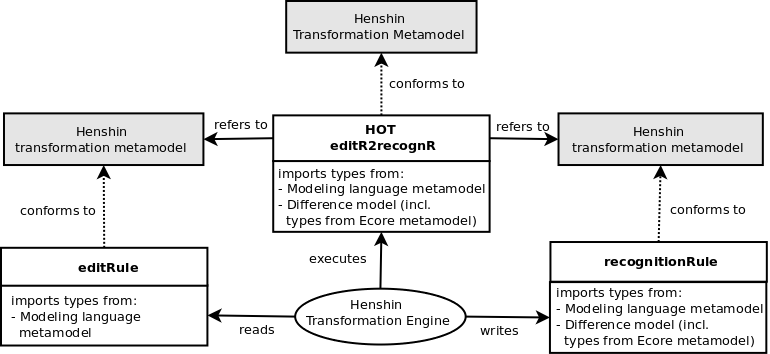
\includegraphics[width=1.0\textwidth]{pic/editR2recognitionR-overview-1.png}
  \caption{Overview: Higher-order transformation \textit{editR2recognR}}
  \label{fig:overview}
\end{figure}

Figure \ref{fig:henshin-metamodel} shows the clipping of the
Henshin transformation metamodel which is relevant in the context
of our transformation domain: 
Two graphs describe the left-hand-side (LHS)
and the right-hand-side (RHS) patterns of a transformation rule, 
respectively.
Parts of a pattern, i.e. nodes and edges, that are mapped via
the respective LHS and RHS nodes are to be found and \textit{preserved} when
a rule is applied to an input model.
Unmapped parts of an LHS pattern are to be found
and \textit{deleted}, unmapped parts of an RHS pattern 
are to be \textit{created}.

\begin{figure}[htb]
  \centering
  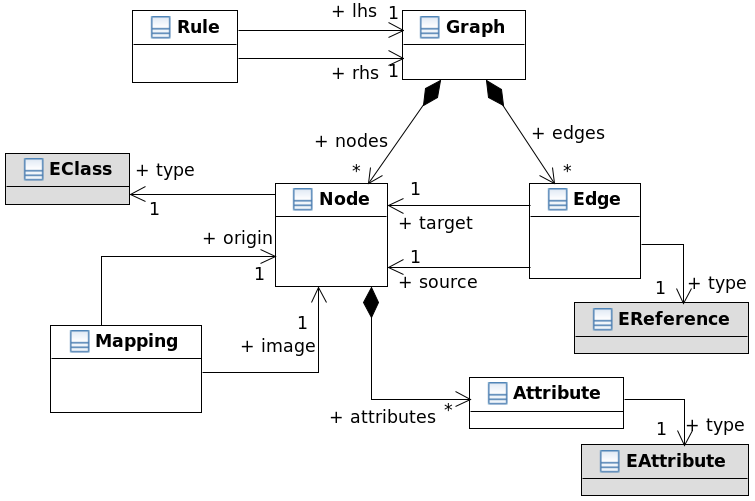
\includegraphics[width=0.7\textwidth]{pic/henshin-metamodel.png}
  \caption{Henshin transformation metamodel}
  \label{fig:henshin-metamodel}
\end{figure}

Nodes, edges and attributes of pattern definitions are further typed over any EMF model.
In terms on an edit rule, this is the metamodel related to a certain modeling language, 
e.g. UML class models, statemachines or any domain-specific language (DSL).
A recognition rule imports additional type definitions:
The semantic lifting transformation works on our
EMF-based representation of model differences.
Thus, graph patterns of recognition rules are typed over 
the \textit{difference model} which is introduced in 
\cite{KeKT2011ASE} and which is worth to briefly recall here.
The structural parts of the difference model are shown
in Figure \ref{fig:diffmodel}.
%, for context-sensitive
%constraints we refer to \cite{KeKT2011ASE}.
Two EMF models \texttt{modelA} and \texttt{modelB} that are
being compared are represented by \texttt{ResourceSets}. 
A \texttt{Difference} is obtained by the three sequential steps
introduced in Section \ref{sec:semantic-lifting}:
\begin{enumerate}

  \item Initially, a matching algorithm populates
the correspondences representing the common parts of model
A and model B. A \texttt{Correspondence} links an \texttt{EObject} of model A 
(\texttt{objA}) to an \texttt{EObject} of model B (\texttt{objB}).
Correspondences between object references are given implicitly by
their corresponding source and target objects.

  \item Subsequently, low-level \texttt{Changes} are instantiated during
difference derivation. We distinguish the following types of 
low-level changes:

\begin{itemize}
\item An \texttt{AttributeValueChange} represents a value change
  of an attribute involving a pair of corresponding objects; \texttt{objA} is
  contained by model A, \texttt{objB} by model B.

\item A change of type \texttt{AddObject} represents the
  insertion of a new object, i.e.\ an object that is contained in
  model B but does not have a corresponding object in model A.
  Analogously, changes of type \texttt{AddReference} represent references
  that have been inserted. 

\item Changes of types \texttt{RemoveObject} and
  \texttt{RemoveReference} represent the inverse of
  changes of types \texttt{AddObject} and
  \texttt{AddReference}, respectively.

\end{itemize} 

  \item Finally, in terms of semantically lifting a model difference, low-level
changes that result from the invocation of a dedicated user-level
edit operation are grouped by \texttt{SemanticChangeSets}.
As each low-level change results from the application of
exactly one edit operation, semantic change sets ideally
provide a complete partitioning of the set of all low-level
changes.

\end{enumerate}


\begin{figure}[htb]
  \centering
  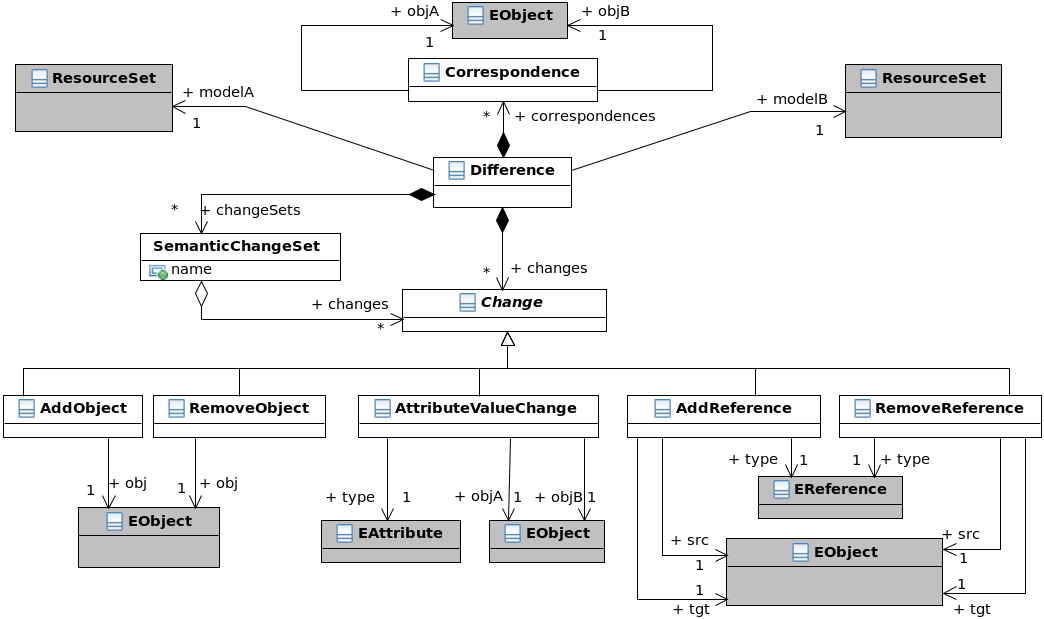
\includegraphics[width=1.0\textwidth]{pic/diffmodel.png}
  \caption{EMF-based difference model}
  \label{fig:diffmodel}
\end{figure}




\section{A By-Example Transformation Specification}
\label{sec:specification}

This section provides a by-example specification of the higher-order transformation \textit{editR2recognR}.
We consider the edit operation ``create generalization'' which
is available for UML class models.
The example is based on the UML metamodel \cite{Superstructure}, 
the part which is relevant for our example is shown in 
Figure \ref{fig:uml-metamodell}.

\begin{figure}[h!]
    \centering
    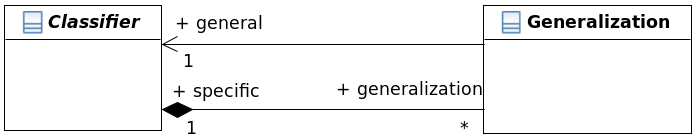
\includegraphics[width=0.6\textwidth]{pic/uml-metamodel.png}
    \caption{Generalizations in the UML metamodel}
    \label{fig:uml-metamodell}
\end{figure}

Figure \ref{fig:sample} (top) shows the Henshin rule
\textit{editR-createGeneralization}, which formally specifies the edit
operation ``create generalization''.
The rule is shown in the graphical syntax of the
Henshin rule editor 
integrating LHS and RHS in a unified diagram. Stereotypes
\texttt{<<create>>}, \texttt{<<delete>>} and \texttt{<<preserve>>} 
are utilized to denote creation, deletion and preservation, 
respectively \cite{JuT2011TTC}.

According to the UML metamodel, generalization relationships are represented
as objects of type \texttt{Generalization}. A generalization is 
owned by the \texttt{specific} classifier of a relationship
and navigates to the more \texttt{general} classifier in the generalization 
hierarchy.
Consequently, \textit{editR-createGeneralization} specifies 
a \texttt{Generalization} object to be created and to be added 
as child of the specific classifier; by the creation of 
containment reference \texttt{generalization}. The general
classifier is referred to via reference \texttt{general} which
is to be created.
The specific and the general classifier are to be preserved 
by the edit rule. They are provided as input parameters
\texttt{s} and \texttt{g}, respectively.

% \tk{Davon könnten wir Gebrauch machen, sollten wir mehr Platz brauchen:
% Please note that the respective \texttt{<<preserve>>}-stereotypes are not shown for
% preserved references in the model pattern of rule ``recognitionR-restrictNav''
% due to space limitations.}
\begin{figure}[h!]
  \centering
  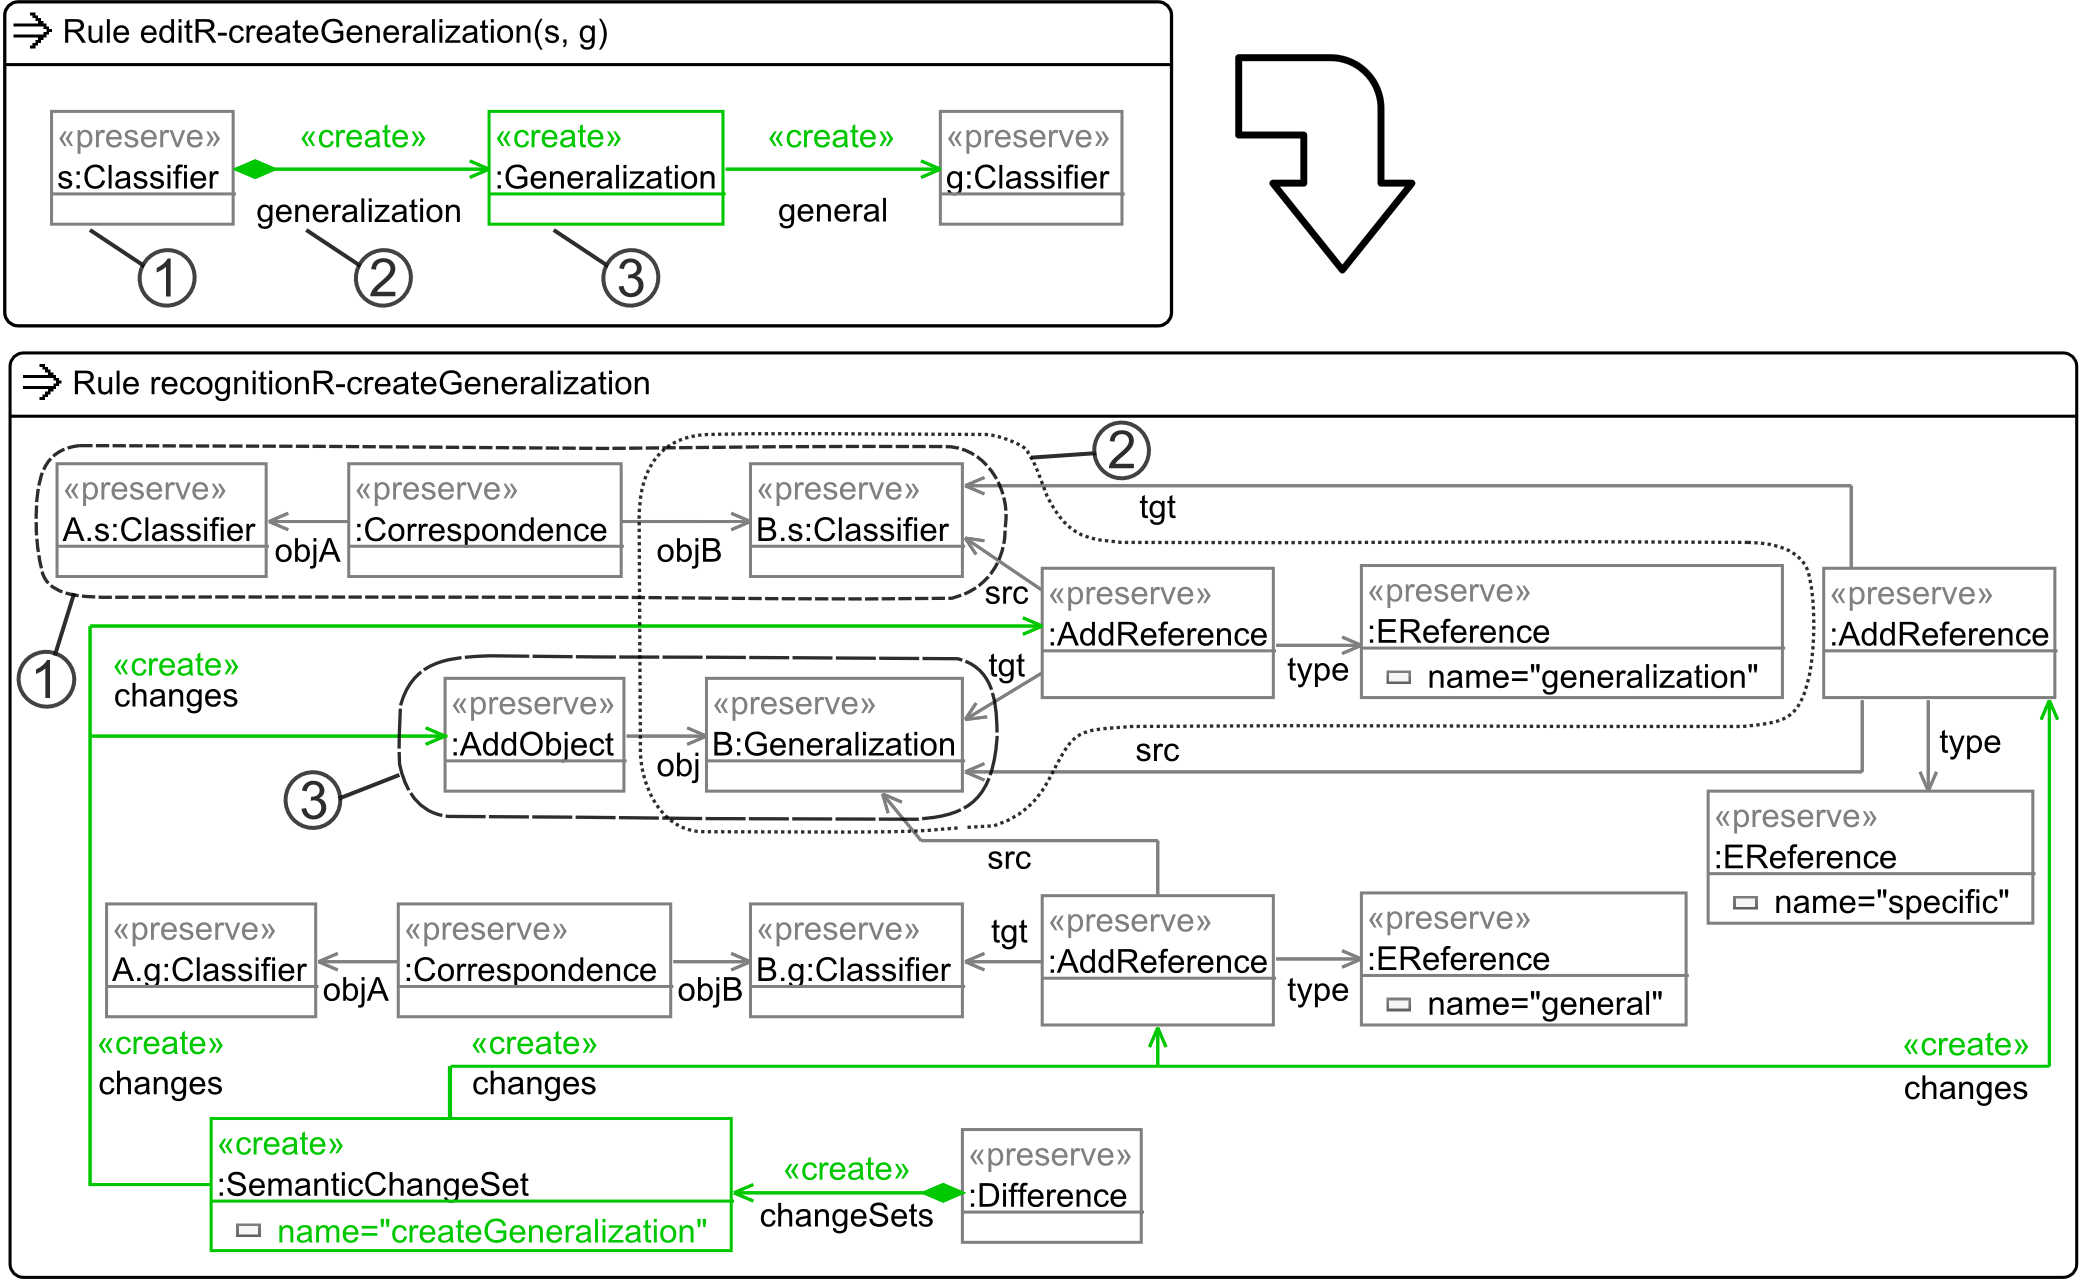
\includegraphics[width=1.0\textwidth]{pic/editR2recognitionR-sample_v02.png}
  \caption{Transformation of sample edit rule \textit{editR-createGeneralization} to corresponding recognition rule \textit{recognitionR-createGeneralization}}
  \label{fig:sample}
\end{figure}

The application of \textit{editR-createGeneralization} to a 
UML class model leads to a characteristic change pattern on 
our EMF-based difference representation.
This change pattern has to be matched
by the corresponding recognition rule
\textit{recognitionR-createGeneralization}, which
is shown by the bottom part of Figure \ref{fig:sample};
the preserved parts of the rule specify the change pattern 
which has to be found.
A change pattern to be matched is composed
of partly overlapping atomic subpatterns, which can be directly
derived from the corresponding edit rule:

\paragraph{Preserve patterns.}
Preserved parts, i.e. nodes and edges, providing the context of an edit rule lead to 
two types of preserve patterns; the \textbf{correspondence pattern}
and the \textbf{preserved reference pattern}:

Model objects which are to be preserved by an edit rule are linked 
by a \texttt{Correspondence} in the difference representation. 
Two instances of the correspondence pattern occur 
in terms of our example. 
They represent the preserved classifiers between which the 
generalization relationship is to be created.
The correspondence pattern which results from the preserved 
specific classifier \textcircled{1} is emphasized
in Figure \ref{fig:sample}.

References which are to be preserved by an edit rule
are not explicitly marked in the difference representation, 
i.e. no direct correspondence links are established between 
the respective references in model A and model B.
However, corresponding references can be identified by their 
context, i.e. corresponding source and target objects. Thus,
a preserved reference pattern usually incorporates two 
correspondence patterns. An instance of this type of 
preserve pattern does not occur in terms of our example.



\paragraph{Atomic change patterns.}
The types of atomic change patterns can be derived from the 
types of low-level changes that can be specified by an edit rule.

Firstly, we consider objects which are to be created or deleted
by an edit rule. In terms of our example,
the \texttt{Generalization} object which is to be created by the
edit rule results in an instance of the \textbf{add object pattern},
which is emphasized and annotated with \textcircled{3} in Figure \ref{fig:sample}; 
the change of type \texttt{AddObject} references the created 
generalization object which is contained by model B. The
inverse low-level change, i.e. an object that
is declared to be deleted by the edit rule, does not occur
in terms of our example. However,
the \textbf{remove object pattern} is structurally equal to 
the add object pattern.
  
Secondly, references can be declared to be created or deleted
by an edit rule.
For example, the reference \texttt{generalization}, which is to be created by
our sample edit rule
\textit{editR-createGeneralization}, results in an instance of
the \textbf{add reference pattern}, which is emphasized and
annotated with \textcircled{2} in Figure \ref{fig:sample}.
As one can see in Figure \ref{fig:sample}, the add reference
pattern \textcircled{2} intersects with the patterns \textcircled{1} and
\textcircled{3}.
% An add reference pattern contains an \texttt{AddReference} change
% providing the information of the difference model; 
% the type of the created reference as well as the source and target
% objects in model B. 
Generally, source and target objects of an add reference pattern are part of
a correspondence pattern or an add object pattern and serve
as ``gluing points'' of the respective pattern intersections.

Two further add reference patterns, which are not explicitly
marked in Figure \ref{fig:sample}, occur in terms of our example.
The first one represents the reference \texttt{general} which is to be 
explicitly created by \textit{editR-createGeneralization}.
The second one represents the reference \texttt{specific}
which is to be implicitly created as it is declared to be
the opposite reference to \texttt{generalization} in
the EMF-based implementation of the UML metamodel. 
Reference pairs that are declared as opposite to each
other need to be specified in one direction only in terms of
edit rules, as the existence of the opposite reference is a 
general EMF constraint.
The \textbf{remove reference pattern}, of which no instance 
occurs in terms of our example,
is structurally equal to the add reference pattern. Gluing points
are provided by a correspondence pattern or a remove object pattern.

Finally, attribute value changes can be induced by edit rules. 
These do usually occur for edit rules which implement typical 
``setter operations''. Thus, no occurrence is provided
by our example.
The object being the owner of a changed attribute is to
be preserved.
The value to which the attribute is to be set is specified by 
the RHS of the edit rule. 
The \textbf{attribute value change pattern} to be detected by 
a corresponding recognition rule consists of an 
\texttt{AttributValueChange} that references the type of the changed 
attribute and links the owner object of model A with the
corresponding attribute owner of model B. 



\paragraph{Semantic lifting.}
The application of a recognition rule semantically 
lifts all low-level changes of a change pattern
by grouping them to a \texttt{SemanticChangeSet}
which represents the invocation of the respective user-level
edit operation. Semantic change sets which are created
by our example recognition rule \textit{recognitionR-createGeneralization} 
consist of four low-level
changes. A semantic change set is finally inserted
into the overall \texttt{Difference}. 



\section{Rule-based Transformation Design}
\label{sec:design-implementation}
This section describes the rule-based design of our implementation of
\textit{editR2recognR} based on EMF Henshin. The transformation algorithm
is structured into five sequential phases which are shown in Figure \ref{fig:mainUnit}.
Each phase produces information which used in the subsequent
one. The design of each phase is described during the remainder
of this section\footnote{The implementation
of all transformation rules and the complete rule application 
strategy are provided at: http://pi.informatik.uni-siegen.de/Projekte/sidiff/pipeline/semantic-lifting/hot/index.htm}. 

\begin{figure}[htbp]
  \centering
  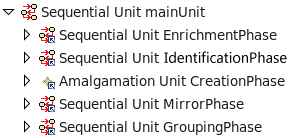
\includegraphics[scale=0.7]{pic/mainUnit.png}
  \caption{Main sequential phases of the transformation algorithm}
  \label{fig:mainUnit}
\end{figure}


As Henshin provides support for in-place transformations only,
a technical helper structure is needed to integrate edit and
recognition rule in a single EMF model. This is the primary purpose
of the intermediate structure which is shown in Figure 
\ref{fig:helper-structure} and implemented in Ecore. 
To setup the transformation, an instance of type \texttt{Edit2Recognition}
is created, which refers to the given input edit rule and the
initially empty output recognition rule, which is also created during
transformation setup time. 

\begin{figure}[htbp]
  \centering
  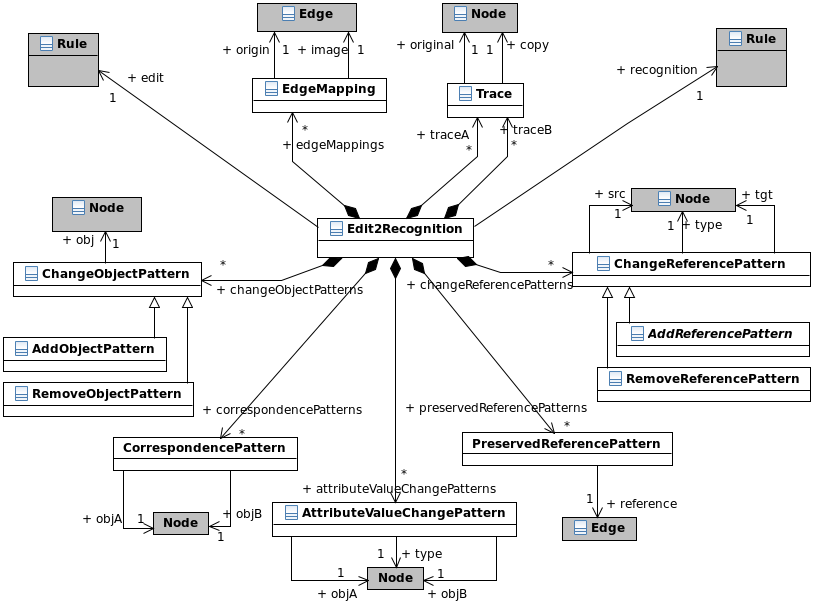
\includegraphics[width=\textwidth]{pic/helper-structure-1.png}
  \caption{Intermediate transformation helper structure}
  \label{fig:helper-structure}
\end{figure}

% \begin{enumerate}
%   \item \textbf{Enrichment phase:} Anreicherung der edit rule
%   \item \textbf{Matching phase:} Change pattern identification
%   \item \textbf{Creation phase:} Change pattern completion
%   \item \textbf{Mirror phase:} Spiegeln isomorpher Teilgraphen
%   \item \textbf{Grouping phase:} Gruppieren der Changes zu SemanticChangeSets
% \end{enumerate}

% The first two of these phases populate further helper information
% of our intermediate transformation structure shown in Figure \ref{fig:helper-structure}. 
% The information is used in terms of the remaining three phases.
% 
% Each phase is implemented by a set of two up to five transformation
% rules; sind unter http://******* dargestellt.
% Rule application strategy (d.h. Rule Scheduling and Location determination)  
% is rather simple: Phasen sequentiell,
% Rules einer Phase können parallel auf alle möglichen
% Matches angewendet werden. \tk{ist das so korrekt?, Umsetzung
% über mittels Units sollte ebenfalls auf die obige WWW-Seite}
% Nachfolgend werden die einzelnen Phasen sowie die
% erzeugten bzw. genutzten Hilfsinformationen näher beschrieben.



\subsection{Enrichment Phase}
In terms of edit rules, reference pairs that are declared as opposite to each
other need to be specified in one direction only (cf. Section \ref{sec:specification}).
In order to implement a consistent derivation of all 
reference-related patterns in later phases, reference pairs which are only
specified partially by the given edit rule are completed. This function is implemented
by the rule \texttt{CreateImplicitEdge}, which can
be applied to all possible matches in parallel, which is 
scheduled by an amalgamation unit with empty 
kernel rule (s. Figure \ref{fig:enrichmentUnit}).

Subsequently, the intermediate structure 
is further populated with helper information facilitating the handling
of preserved references: The information if a reference is to be
preserved by an edit rule is not explicitly available.
Thus, the rule \texttt{MapPreservedEdge} identifies preserved
references by means of their context, i.e. source and
target nodes which are mapped from LHS to RHS. 
The information is made explicit by an \texttt{EdgeMapping} which maps
the \texttt{origin} edge of an edit rule LHS to the \texttt{image} edge of the edit rule RHS
(s. Figure \ref{fig:helper-structure}).
\texttt{MapPreservedEdge} can be applied to all possible matches
in parallel (s. Figure \ref{fig:enrichmentUnit}).

\begin{figure}[htbp]
  \centering
  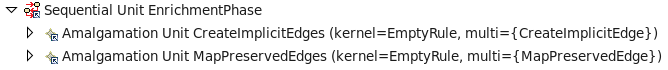
\includegraphics[scale=0.7]{pic/enrichmentUnit.png}
  \caption{Rule application strategy for enrichment phase}
  \label{fig:enrichmentUnit}
\end{figure}

\subsection{Identification Phase}
The identification phase analyzes the edit rule and identifies all
atomic preserve and change patterns which result from its application.
For each change pattern that is identified, a helper object of 
the respective type of atomic pattern is instantiated and
populated with the relevant information 
(cf. Figure \ref{fig:helper-structure}).

Usually, several atomic change patterns are partly overlapping
to form a complete change pattern which is induced by an edit operation invocation.
The ``gluing points'' are provided by objects that are
preserved, deleted or added. Gluing points that are to be matched
by a recognition rule are created by the same transformation rules 
that create the helper objects which are used to identify
atomic change patterns in an output rule;
\texttt{IdentifyCorrespondencePattern}, 
\texttt{IdentifyAddObjectPattern} and \texttt{IdentifyRemoveObjectPattern}, 
respectively (s. ``IdentificationPhase01'' in Figure \ref{fig:identification-and-creationUnit}, left).
These rules additionally create \texttt{Traces} from nodes of
the edit rule to their counterparts in the recognition rule.
Tracing information is necessary in order to correctly identify the gluing points
for all overlapping atomic change patterns which are identified
by the remaining rules of the identification phase, applied
to all possible matches in parallel in ``IdentificationPhase02''.
% \texttt{IdentifyPreservedReferencePattern},
% \texttt{IdentifyAddReferencePattern},
% \texttt{IdentifyRemoveReferencePattern}, and
% \texttt{IdentifyAttributeValueChangePattern}
% Each rule can be applied to all possbile matches in 
% parallel. The overall rule application strategy of the identification phase
% is shown in Figure \ref{fig:identification-and-creationUnit}.

If modeling language types are referenced multiple times by an edit rule, 
the schematic creation of change patterns may lead to
multiple occurrences of recognition rule nodes representing
the types. These have to be finally reduced to a single occurrence 
for each type due to the following reason: 
During semantic lifting, each type of the modeling language is
represented by a single object of the respective metamodel.
As recognition rules are injectively matched into the
EMF-based representation of a given difference, multiple occurrences of these
type objects have to be removed. This is achieved by
a repeated application of the rules \texttt{RemoveDuplicatedEReferenceTypes}
and \texttt{RemoveDuplicatedEAttributeTypes} which terminate
as soon as all duplicates are removed (s. Figure \ref{fig:identification-and-creationUnit}, left).

 
\begin{figure}[h!]
	\centering
	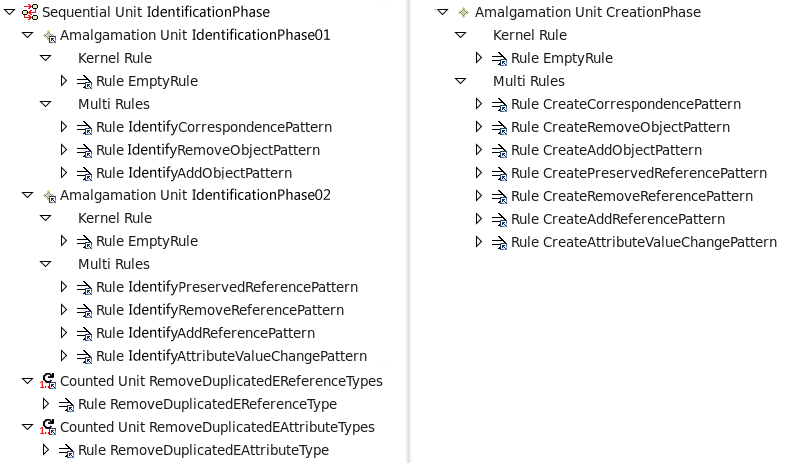
\includegraphics[scale=0.6]{pic/IdentificationAndCreateUnit.png}
	\caption{Rule application strategy for identification phase (left) and creation phase (right)}
	\label{fig:identification-and-creationUnit}
\end{figure}



\subsection{Creation Phase}
The creation phase completes the atomic change patterns that 
have been identified and been partly created by the identification phase: 
Nodes representing the low-level changes oy type \texttt{Correspondence},
\texttt{AddObject}, \texttt{RemoveObject}, \texttt{AddReference} and \texttt{RemoveReference} 
are created and embedded into 
the change patterns.
As these change objects have no references across each other,
no sequential dependencies have to be considered. Thus, all
rules of the creation phase can be applied in parallel to
all possible matches (s. Figure \ref{fig:identification-and-creationUnit}, right).




\subsection{Mirror Phase}

Please note that up to this state of the transformation,
only the LHS part of a change pattern to be
matched and preserved by the output recognition rule have
been created. This keeps transformation rules
of the identification and creation phase at a manageable size.
The RHS part of a change pattern, which is isomorphic
to the RHS part, is created during the mirror phase.
The rule \texttt{MirrorNodesLHStoRHS} simply copies all nodes
of the LHS to the RHS of the recognition rule and
instantiates the respective node \texttt{Mappings} (cf. Figure \ref{fig:henshin-metamodel}).
Afterwards, attributes and edges can be copied to the LHS
by the rules \texttt{MirrorAttributeLHStoRHS} and \texttt{MirrorEdgesLHStoRHS}
in parallel (s. Figure \ref{fig:mirrorUnit}).

\begin{figure}[htbp]
  \centering
  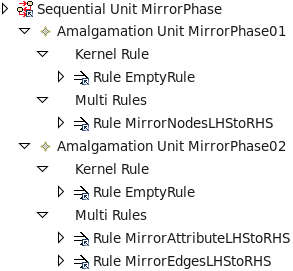
\includegraphics[scale=0.7]{pic/mirrorUnit_v02.png}
  \caption{Rule application strategy for mirror phase}
  \label{fig:mirrorUnit}
\end{figure}

\subsection{Grouping Phase}
Finally, the SemanticChangeSet to be created by the recognition
rule has to be instantiated and to be connected with all 
low-level change nodes of the atomic change patterns. The name
of the semantic change set is derived from the name of
the input edit rule.

\begin{figure}[htbp]
  \centering
  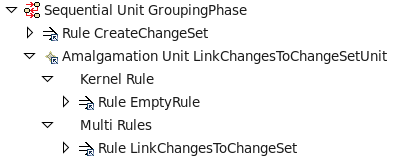
\includegraphics[scale=0.7]{pic/groupingUnit.png}
  \caption{Rule application strategy for grouping phase}
  \label{fig:groupingUnit}
\end{figure}

% \section{Evaluation}
% 
% \tk{Ganz weg lassen..?}
% 
% Diskussion:
% Was wollen mit einer Evaluation zeigen, die Korrekhteit des Transformators (1)..?, inwieweit der Ansatz an sich trägt und zur Verbesserung der Modellqualität beitragen kann (2)..?, den Implementierungsaufwand für die HOT in Henshin messen (3)..?
% 
% \begin{enumerate}
%  
%  \item Wiederdurchführung der Evaluation aus ASE-Papier mit generierten Recogn.Rules. Basis: EditRules von Michaela Rindt. Diese basieren allerdings auf unserem hausinternen UML-Metamodell. Zu erwarten sind also:\\
% 	- gleiche Ergebnisse was die erkannten Change Sets angeht\\
% 	- Allerdings andere Werte für Metriken da anderes Differenzmodell und strukturell anderes UML-metamodell als das für ASE-Papier verwendete Eclipse UML2-Metamodell
% % Nevertheless, basic model edit operations lead to some complexity on
% % the level of abstract syntax graphs (ASG), since the UML metamodel defines many redun-
% % dant or mutually dependent data items in an ASG.
% 
%  \item  Die von Manuel durchgeführte Evaluation: Historie von GMF-Modellen
%  
%  \item Vergleich mit Java-Implementierung der Transformation; Metriken, welche Aufwände jeweils investiert werden müssen ?
%  
% \end{enumerate}


\section{Comparison to a Direct Manipulation Approach}
\label{sec:java-comparison}
A very brief specification sketch of designing \textit{editR2recognR} as 
direct manipulation approach in imperative logic \cite{CzH2006IBM} is 
given in \cite{KeKT2011ASE}. We implemented the direct manipulation in 
Java\footnote{The source code is freely available at: http://pi.informatik.uni-siegen.de/Projekte/sidiff/pipeline/semantic-lifting/hot/index.htm}
independently from our implementation in Henshin.
A comparison of both implementation design reveals, that
almost the same ``functions'' are used (s. Table \ref{tab:java-comparison}). 
% With respect to function names, Java method names are usually
% plural, whereas Henshin rule names are singular. This is
% due to the fact, that ``for each iterations'' are implemented
% in Java as loops within the respective methods; the corresponding
% Henshin rules are embedded in amalgamation units realizing
% a parallel processing.


A design pattern that can be observed for the Henshin-based 
realization is the sequential enrichment of helper data.
This is used to ``emulate'' procedure calls providing
return values of complex data types.
For example, the creation of atomic change patterns can
be decomposed into two logical functions: Firstly, their
cause have to be detected by an analysis of the edit rule
before the pattern specification is actually synthesized within
the recognition rule. For a concrete type of atomic change pattern,
e.g. the correspondence pattern, this is implemented straight-forward
in Java: The method \texttt{createCorrespondencePatterns()}
simply calls the utility method \texttt{getLHSIntersectRHSNodes()}, 
which implements a query that returns the ``preserved'' nodes of an
edit rule. In Henshin, the same utility function is realized 
by the rule \texttt{IdentifyCorrespondencePattern} which 
creates helper data being later used by the rule 
\texttt{CreateCorrespondencePattern}.
%Another example: Anlegen von Hilfsdaten auch durch MapPreservedEdge, was in Java durch utility method isEdgeMapped gelöst wird.

\begin{table}[htb]
\centering
\caption{Comparison to a direct transformation approach implemented in Java}

\begin{tabular}{llcl}
\toprule
\textbf{Phase} \ & \textbf{Henshin rule}  & & \textbf{Java method / utility class} \\
\cmidrule{1-4}
EP: & CreateImplicitEdge & & createImplicitEdges() \\
& MapPreservedEdge & & isEdgeMapped() \\

IP: & MatchCorrespondencePattern & & getLHSIntersectRHSNodes() \\
& IdentifyAddObjectPattern & & getRHSMinusLHSNodes() \\
& \multicolumn{1}{c}{\vdots} & & \multicolumn{1}{c}{\vdots} \\
& RemoveDuplicatedEReferenceTypes & & -  \\
& RemoveDuplicatedEAttributeTypes & & -  \\

CP: & CreateCorrespondencePattern & & createCorrespondencePatterns()  \\
& CreateAddObjectPattern & & createAddObjectPatterns()  \\
& \multicolumn{1}{c}{\vdots} & & \multicolumn{1}{c}{\vdots} \\

MP: & MirrorNodesLHStoRHS & & - \\
& MirrorAttributeLHStoRHS & & - \\
& MirrorEdgesLHStoRHS & & - \\

GP: & CreateChangeSet & & \multirow{2}{*}{createChangeSet()} \\
& LinkChangesToChangeSet & & \\
\cmidrule{2-4}
& - & & ModelHelper.java \\
& - & & ModelHelperEx.java \\
& - & & NodePair.java \\
\bottomrule
\end{tabular}
  \label{tab:java-comparison}
\end{table}

Two Henshin rules that do not have any corresponding Java method 
implementing the same functionality are 
\texttt{RemoveDuplicatedEReferenceTypes} and \texttt{RemoveDuplicatedEAttributeTypes} 
In terms of the Java implementation, duplicate type nodes are never created
because a simple condition checks whether these type nodes 
already exist when an atomic change pattern is synthesized
(cf. lines 258, 340 and 405 in \texttt{EditRule2RecognitionRule.java}).
In Henshin, the same behavior could be realized 
using conditional units and implementing a loop processing instead of a 
parallel creation of atomic change patterns. In this case,
\texttt{RemoveDuplicatedEReferenceTypes} and \texttt{RemoveDuplicatedEAttributeTypes} 
would be obsolete. However, the total number of rules needed by 
this transformation design would be significantly
higher: For each rule of the identification phase, three
rules would be required, i.e. ``if rule'', ``then rule'' and
``else rule'' of the respective conditional unit.

Further Henshin rules which have no corresponding Java methods implementing the same function are
\texttt{MirrorNodesLHStoRHS},
\texttt{MirrorAttributeLHStoRHS} and
\texttt{MirrorEdgesLHStoRHS}, which facilitate the output rule
synthesis; initially only the LHS
of the output recognition rule has to be synthesized which is later mirrored onto
the RHS. In Java, the consistent handling of LHS and RHS graphs of a 
recognition rule is implemented using data abstractions. 
These data abstractions provide a high-level API to manipulate 
internal, fine-grained representations of Henshin rules. For example, 
the utility function \texttt{createPreservedNode()} of class 
\texttt{HenshinRuleAnalysisUtilEx} and the wrapper class \texttt{NodePair} are provided 
in order to encapsulate preserved nodes: Creation and 
management of LHS node, RHS node and the according mapping 
are handled transparently to a programmer.



\section{Conclusion}
\label{sec:conclusion}
In this paper, we introduced a new application of higher-order
model transformations: Complex recognition rules, which are necessary to
semantically lift low-level model differences into representations
of user-level edit operations, are generated from their corresponding
edit rules, which are much easier to design. In some cases,
edit rules are even readily available, e.g. for UML class
models \cite{RiKKP11TechRep}.

None of the categories of the classification scheme 
for higher order transformations given in \cite{TiJFCB2009ECMDA} matches
perfectly to our application. The most closely related
category is transformation type c) as it requires
input \textit{and} output models to be model transformations themselves.
However, our application does not compose or decompose transformations.
Thus, the proposed design patterns \textit{internal} and \textit{external (de-)composition}
are not applicable to our use case. 

Instead, our rule-based transformation design based on EMF Henshin
reveals that patterns that are known form procedural programming
can help to structure the transformation design.
Utility functions providing structurally complex return types 
can be realized by the definition of an intermediate helper 
structure. This pattern can be generalized and applied to all
types of rule-based transformations. 
Two other patterns that are used specifically apply to
higher-order transformations: Firstly, providing the explicit 
information of preserved edges facilitates queries on the 
rule serving as input of the HOT. Secondly, the mirroring of preserved parts from LHS to RHS facilitates the output rule synthesis. The second pattern is very specific to the transformation domain described in this paper as most parts of a recognition rule are preserved. However, it can be generalized to all HOTs generating transformation rules that are mainly used for pattern matching purposes.


%
% ---- Bibliography ----
%
\begin{thebibliography}{W}

\bibitem {Arendt2010} Arendt, T.; Biermann, E.;
Jurack, S.; Krause, C.; Taentzer, G.: Henshin: Advanced
Concepts and Tools for In-Place EMF Model Transformations;
in: Proc. Intl. Conf. Model Driven Engineering Languages
and Systems (MoDELS 2010); Springer, LNCS 6394;
2010

\bibitem{BeE2009MBSE} Bendix, L.; Emanuelsson, P.:
Collaborative Work with Software Models - Industrial Experience
and Requirements; Proc. Intl. Conf. Model-Based Systems
Engineering, Haifa; 2009

\bibitem{CzH2006IBM}
Czarnecki, K; Helsen, S.:
Feature-based survey of model transformation approaches;
p.621-646 in: IBM Systems Journal, Vol. 45, No. 3; 2006

\bibitem{EMFC} EMF Compare;
\url{http://www.eclipse.org/emf/compare}

\bibitem{EMF} EMF: Eclipse Modeling Framework;
\url{http://www.eclipse.org/emf}

\bibitem{EMFRefactor} EMF Refactor;
\url{http://www.eclipse.org/modeling/emft/refactor/}

\bibitem{GiW2009SoSyM}
Giese, H.; Wagner, R.:
From model transformation to incremental bidirectional model synchronization
p.21-43 in: Software and Systems Modeling, Vol. 8, No. 1; 2009

\bibitem{Henshin} Henshin;
\url{http://www.eclipse.org/modeling/emft/henshin/}

\bibitem{KM3}
Jouault, F.; Bézivin, J.: 
KM3: a DSL for Metamodel Specification;
p. 171—185 in: Proc. of 8th IFIP International Conference on Formal Methods for Open Object-Based Distributed Systems;
LNCS; 2006

\bibitem{JuT2011TTC}
Jurack, S; Tietje J.:
Solving the TTC 2011 Reengineering Case with Henshin;
p. 181-203 in: Proc. of the 5th Transformation Tool Contest (TTC); 
EPTCS; 2011

\bibitem {KeKT2011ASE} Kehrer, T.; Kelter, U.;
Taentzer, G.: A Rule-Based Approach to the Semantic
Lifting of Model Differences in the Context of Model
Versioning; p.163-172 in: Proc. 26th IEEE/ACM Intl. Conf.
Automated Software Engineering (ASE 2011); ACM;
2011

\bibitem {Ke2010SE} Kelter, U.:
Pseudo-Modelldifferenzen und die Phasenabhängigkeit von
Metamodellen; p.117-128 in: Proc. Software Engineering
(SE 2010); GI LNI 159; 2010

\bibitem {KeS2008CVSM} Kelter, U.; Schmidt, M.:
Comparing State Machines; p.1-6 in: Proc. ICSE Workshop on
Comparison and Versioning of Software Models (CVSM 2008);
ACM; 2008

\bibitem{MDAExplained}
Kleppe, A.;Warmer, J.; Bast, W.:
MDA Explained, The Model Driven Architecture: Practice and Promise, 
Addison-Wesley, 2003

\bibitem {KoRPP2009CVSM} Kolovos, D.S.; Ruscio,
D.D.; Pierantonio, A.; Paige, R.F.: Different Models for
Model Matching: An Analysis Of Approaches To Support Model
Differencing; p.1-6 in: Proc. 2009 ICSE Workshop on
Comparison and Versioning of Software Models; IEEE; 2009

\bibitem{MDA}
MDA Guide Version 1.0.1; OMG, http://www.omg.org; 2003

\bibitem{QVT}
OMG: MOF Query/View/Transformation;
\url{http://www.omg.org/spec/QVT/1.0/}; 2008

\bibitem{Superstructure}
OMG: Unified Modeling Language; 
Superstructure specification version 2.3; 
\url{http://www.omg.org/spec/UML/2.3/Superstructure/PDF/}; 2010




\bibitem {RiKKP11TechRep}
Rindt, M.; Kehrer, T.; Kelter, U.; Pietsch, P.: Henshin
Rules for Edit Operations in Class Diagrams; Technical
Report, QuDiMo Project, University of Siegen, 
\url{http://pi.informatik.uni-siegen.de/qudimo/download/RiKKP2011.pdf};
2011

% \bibitem{sidiff} SiDiff Project;
% http://www.sidiff.org

\bibitem{TiJFCB2009ECMDA}
Tisi, M.; Jouault, F.; Fraternali, P.; Ceri, S.; Bézivin J.:
On the Use of Higher-Order Model Transformations;
p.18-33 in: Proceedings of the 5th European Conference on
Model-Driven Architecture Foundations and Applications (ECMDA);
Springer; 2009


\end{thebibliography}

\end{document}
